% вторая часть

\section{Сравнение эксплуатационных характеристик аналоговой и цифровой видеосистем}

\subsection{Основные сведения}

Аналоговый сигнал -- сигнал данных, у которого каждый из представляющих параметров описывается функцией времени и непрерывным множеством возможных значений \cite{analogDes}.
Значения аналогового сигнала произвольны в каждый момент времени, поэтому он может быть в принципе представлен как некая непрерывная функция (зависящая от времени как от переменной) либо как кусочно-непрерывная функция времени \cite{analog}.

Цифровой сигнал -- сигнал, который можно представить в виде последовательности дискретных (цифровых) значений (рис. \ref{fig:anVSdig}) \cite{digital}.

\begin{figure}[H]
	\centering
	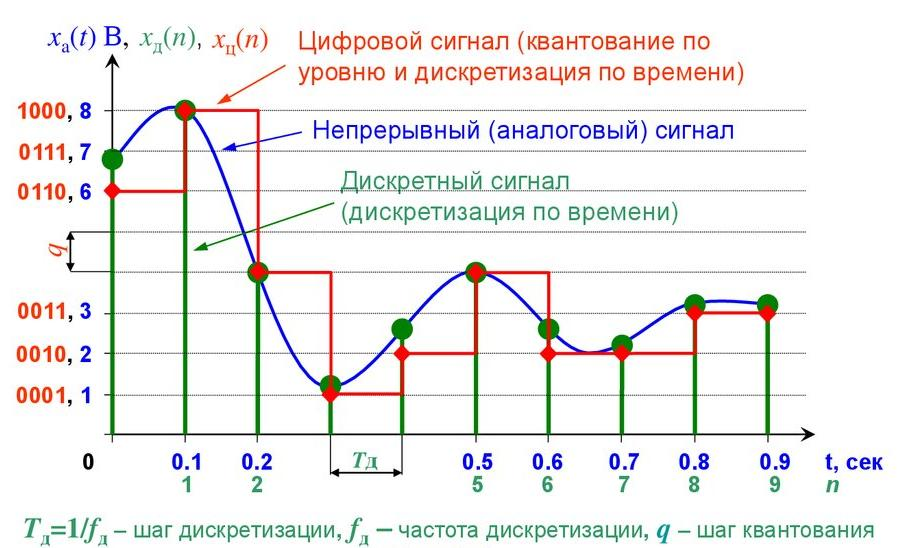
\includegraphics[width=0.7\linewidth]{pics/anVSdig}
	\caption{ Виды сигналов 
	}
	\label{fig:anVSdig}
\end{figure}

В ходе передачи цифрового видеосигнала получаемая от камеры информация кодируется в формат кодека (в большинстве случаев — h.264), чтобы видео помещалось в полосу пропускания Wi-Fi \cite{kodec}. 

Полоса пропускания — диапазон частот, в пределах которого амплитудно-частотная характеристика (АЧХ) акустического, радиотехнического, оптического или механического устройства достаточно равномерна для того, чтобы обеспечить передачу сигнала без существенного искажения его формы \cite{propusk}.

Согласно теореме Шеннона-Хартли определенное количество информации может быть передано по заданной полосе пропускания в присутствии шума. Увеличение пропускной способности увеличивает количество информации, которая передается в течение заданного времени \cite{shenon}.

В случае цифровых видеосистем ширина используемой полосы пропускания существенно определяет качество изображения и задержку. При использовании узкой полосы пропускания цифровая видеосистема может либо отправить сигнал в высоком разрешении с увеличенной задержкой, либо снизить качество видео, чтобы уменьшить задержку. Качество видео может быть снижено путем снижения разрешения или сжатия изображения \cite{profpv}.

Цифровые системы требуют большой полосы пропускания для оптимальной работы. В стандартах связи ширина полосы строго привязана к используемому диапазону частот и сетке каналов. Чтобы обойти ограничения выбранного диапазона по ширине канала некоторые системы осуществляют динамическую перестройку частоты во время работы. Это позволяет передатчикам переключаться на неиспользуемые частоты, чтобы максимизировать доступную полосу пропускания.

Закодированный сигнал посылается по каналу связи. В результате принимаемый сигнал декодируется и становится принимаемым сообщением.  
Так как используется алгоритм сжатия из нескольких кадров, в случае помех или слабого сигнала, пропадают целые кадры или сегменты кадров \cite{profpv}.

Аналоговый сигнал при приеме в FPV оборудовании не нуждается в декодировании, поскольку уже находится в стандартном формате PAL или NTSC \cite{shenon}. Однако при попытке отобразить этот сигнал на компьютере необходимо произвести ЦАП. Доступные модули для получения и преобразования сигнала являются медленными, а разработка собственного не целесообразна в рамках данного проекта.

\subsection{Практические результаты}

В проделанной ранее научно-исследовательской работе \cite{nir} был получен следующий результат:
вес камеры и видеопередатчика с антенной составляли 12~г; задержка аналогового видеосигнала была 217 мс (рис. \ref{fig:time}).

\begin{figure}[H]
	\centering
	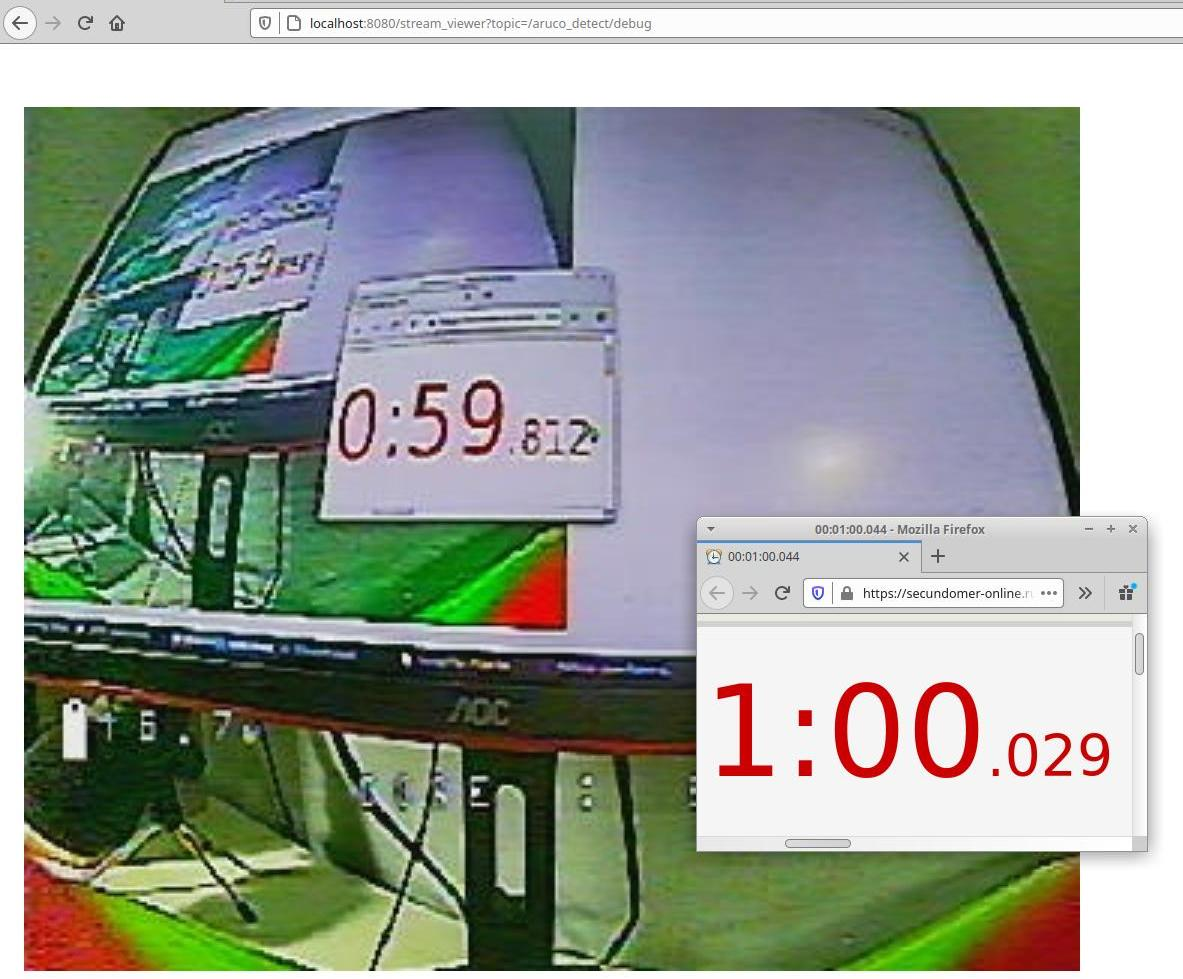
\includegraphics[width=0.5\linewidth]{pics/time}
	\caption{ Задержка аналогового видео
	}
	\label{fig:time}
\end{figure}

В первой части данной работы был собран модуль AirPi, состоящий из bec 5В, RPi Zero V1.3 камеры и микрокомпьютера Raspberry Zero W; общий вес составляет 15~г. Задержка цифрового видеосигнала 145 мс (рис. \ref{fig:photo2}).

\begin{figure}[H]
	\centering
	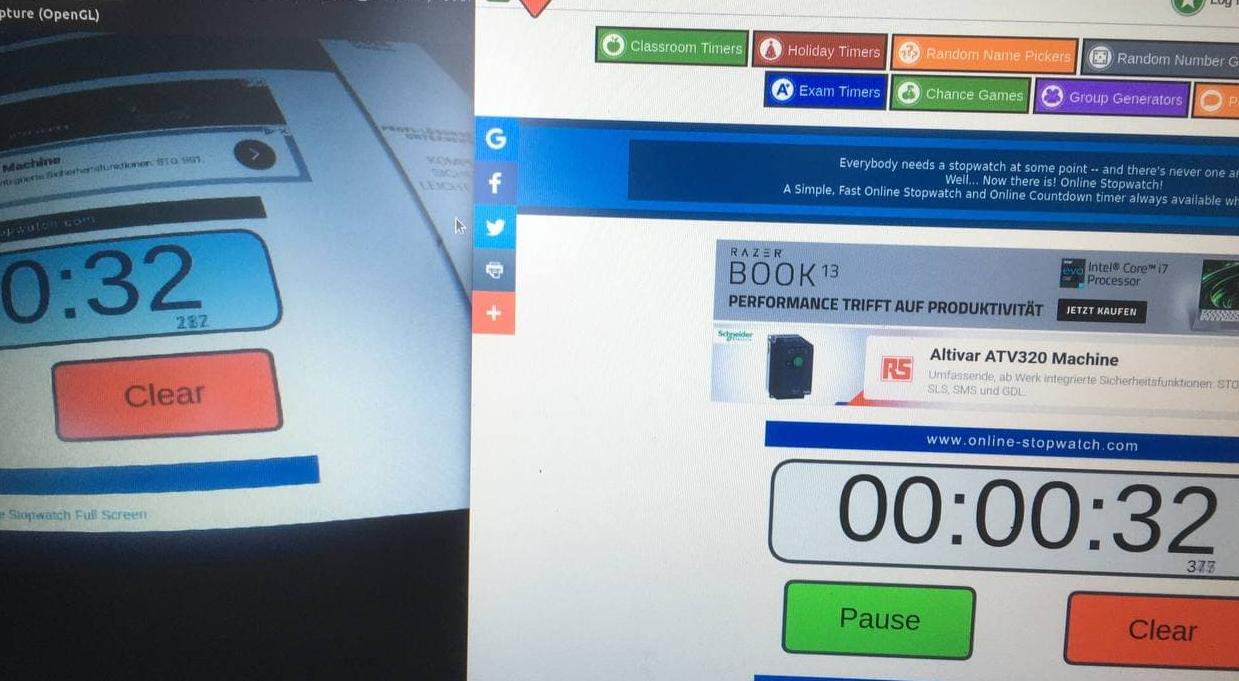
\includegraphics[width=0.5\linewidth]{pics/photo2}
	\caption{ Задержка цифрового видео
	}
	\label{fig:photo2}
\end{figure}

Данный результат получен на настройках по умолчанию и потенциально для уменьшения задержки мы можем снизить разрешение, вплоть до 480*320. Такое разрешение используется на COEX clover для анализа навигационных маркеров. Также исходя из информации репозитория Open.HD, можно уменьшить задержку до 110 мс, сменив оборудование воздушного модуля, но тем самым увеличив вес. 
Текущий полученный результат уже значительно лучше результата аналоговой видеосистемы, что позволяет перейти к его тестированию и осуществить более точную настройку уже в процессе тестирования.